%%%%%%%%%%%%%%%%%%%%%%%%%%%%%%%%%%%%%%%%%%%%%%%%%%%%%%%%%%%%%%%%%%%%%%%%%%%%%%%
%
% results
% Copyright (c) 2010 by tilo.mueller@rwth-aachen.de
% 
%%%%%%%%%%%%%%%%%%%%%%%%%%%%%%%%%%%%%%%%%%%%%%%%%%%%%%%%%%%%%%%%%%%%%%%%%%%%%%%

\chapter{Ergebnisse}

Die Umfrage ergab 856 vollständig ausgefüllte Fragebögen. Dazu 164 nicht vollständig ausgefüllte, die laut dem Feedback Feld teilweise auf das Fehlen eines Zurück-Knopfes zurückzuführen sind, aber wohl eventuell auch einfache Abbrüche waren.

\section{Demographie}
Von den 856 Teilnehmern waren 204 (23,83\%) weiblich, 613 (71,61\%) männlich und 39 haben keine Angabe zu ihrem Geschlecht abgegeben. Die hohe Anzahl an männlichen teilnehmern liegt vermutlich daran, dass die Umfrage über den Email-Verteiler der Technischen Fakultät der Universität Erlangen-Nürnberg verteilt wurde, welche einen höheren Männer- als Frauenanteil hat.
Das durchschnittliche Alter beträgt 24.99 Jahre mit einer Standardabweichung von 9.23 Jahren. Das Maximum ist 99 Jahre und das Minimum 0 Jahre, wobei dies wohl beides Fehler sind - das Minimum könnte durch ein nicht ausgefülltes Feld entstanden sein, wohingegen die Person die das Maximum eingegeben hat mir persönlich gesagt hat dass dies ein Fehler war. Das untere Quartil ist 20, das Mittlere 23 und das Obere 26.
Interessant ist, dass trotz des niedrigen Wertes und der geringen Standardabweichung dennoch einige Fragebögen im Altersbereich von 45 bis 77 liegen. Diese müssen eventuell in der weiteren Auswertung gesondert betrachtet werden - denn selbst wenn ihre Anzahl nicht für statistisch exakte Aussagen reicht könnten hier dennoch interessante Ergebnisse gefunden werden.
Die nächste Frage fragte nach dem höchsten bisher erreichten Schulabschluss. Hier zeigt sich dass ein Großteil der Teilnehmer entweder gerade studiert oder bereits einen Abschluss im Studium erreicht hat. Abitur und Bachelor/Master/Diplom zusammen geben über 90\% der Teilnehmer ab. Dagegen sind Hauptschulabschluss und Realschulabschluss zusammen nur knapp über 5.73\%, was die Relevanz der Umfrageergebnisse ein wenig einschränkt, da sie nicht als allgemeingültig angesehen werden können sondern nur für einen speziellen Teil der Bevölkerung gelten. In einer zukünftigen Arbeit zu diesem Thema sollten eventuell speziell die Gruppen "Kein Abschluss", "Hauptschulabschluss" und "Realschulabschluss" betrachtet werden.
\begin{figure}[H]
\centering
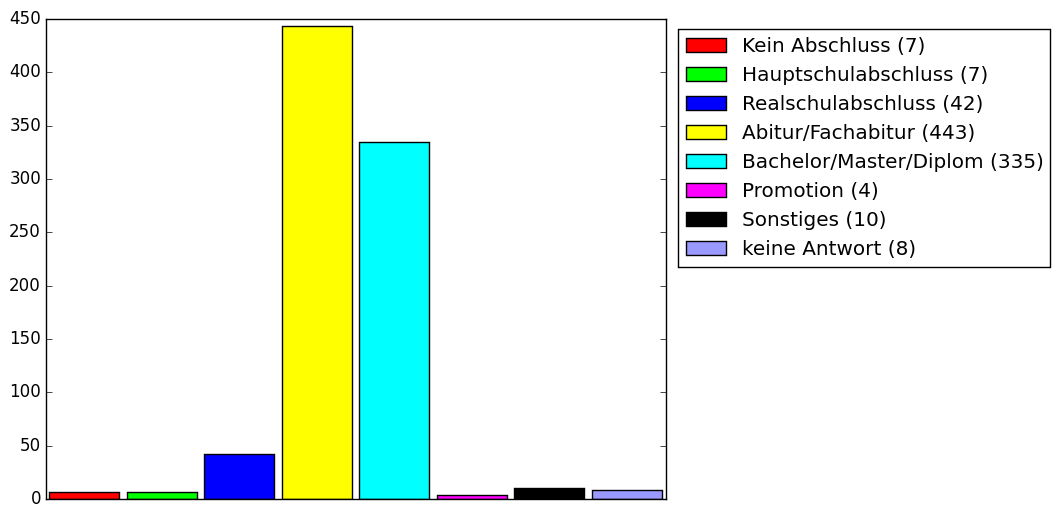
\includegraphics[scale=0.55]{images/schulabschluss}\\
\caption{Höchster Schulabschluss}\label{schulabschluss}
\end{figure}
Auch die folgende Frage zeigt das selbe Problem auf - 76.99\% der Teilnehmer (659) waren zum Zeitpunkt des Ausfüllens Studenten. Dahingegen sind nur 1.99\% in Ausbildung und 14.84\% berufstätig.
Das arithmetische Mittel der selbst eingeschätzten Informatikkenntnisse liegt auf einer Skala von 1 (keine) bis 5 (sehr hohe) bei 3.26. Dass dieser Wert sehr nah an dem zu erwartenden Mittelwert von 3.0 liegt deutet darauf hin, dass die Umfrage trotz der fehlenden Gruppe an Realschülern und Hauptschülern dennoch Relevanz hat. Der größte Anteil hat mit 31.40\% einen Wert von 3 angegeben, kurz darauf folgen Kenntnisse von 4 mit 28.22\% und von 2 mit 24.20\%. Ein größerer Unterschied von über 10\% liegt zwischen denen die den höchsten Wert wählten (13.46\%) und denen die den niedrigsten Wert wählten (2.72\%).
Diese Statistik verschiebt sich stark, wenn man die Frage nach den Kenntnissen in der IT-Sicherheit betrachtet. Hier liegt das arithmetische Mittel bei 2.63, was um 0.63 niedriger ist als das arithmetische Mittel der IT Kenntnisse. Hier liegt das Maximum mit 30.86\% bei einem Wert von 2, Antwortmöglichkeit 3 und 1 haben 29.80\% respektive 16.84\%. Der Unterschied zwischen der Anzahl der Teilnehmer die mit 1 geantwortet haben und denen die mit 5 geantwortet haben liegt aber auch hier mit 12.13\% nicht sehr weit von dem Abstand aus der letzten Frage weg.
Die Ergebnisse dieser Frage korrelieren mit der nächsten Frage: 77.45\% der Teilnehmer haben keinen Bildungsabschluss in der Informatik oder einem anderen IT-nahem Fachbereich.

\section{Hypothesen}

Schon aus den ersten Fragen der Umfrage wird ersichtlich dass Google Dienste sehr aktiv genutzt werden. Auf "Wie aktiv nutzen Sie die folgenden Dienste? Google Suche:" antworteten fast 90% mit 4 und 5, davon sind 73.71% bei der 5 angesiedelt. Auch nutzen über die Hälfte der Umfrageteilnehmer (58.88%) Android mit einer Aktivität von 4 oder 5.

\section{Forschungsfragen}

\section{Sonstiges}
